%%%%%%%%%%%%%%%%%%%%%%%%%%%%%%%%%%%%%%%%%
% University/School Laboratory Report
% LaTeX Template
% Version 3.1 (25/3/14)
%
% This template has been downloaded from:
% http://www.LaTeXTemplates.com
%
% Original author:
% Linux and Unix Users Group at Virginia Tech Wiki
% (https://vtluug.org/wiki/Example_LaTeX_chem_lab_report)
%
% License:
% CC BY-NC-SA 3.0 (http://creativecommons.org/licenses/by-nc-sa/3.0/)
%
%%%%%%%%%%%%%%%%%%%%%%%%%%%%%%%%%%%%%%%%%

%----------------------------------------------------------------------------------------
%	PACKAGES AND DOCUMENT CONFIGURATIONS
%----------------------------------------------------------------------------------------

\documentclass{article}

\usepackage{graphicx} % Required for the inclusion of images
\usepackage{minted}

\setlength\parindent{0pt} % Removes all indentation from paragraphs

\renewcommand{\labelenumi}{\alph{enumi}.} % Make numbering in the enumerate environment by letter rather than number (e.g. section 6)

%\usepackage{times} % Uncomment to use the Times New Roman font

%----------------------------------------------------------------------------------------
%	DOCUMENT INFORMATION
%----------------------------------------------------------------------------------------

\title{In the name of God \\ Database Lab \\ Spring 2016} % Title

\author{Iman \textsc{Tabrizian}} % Author name

\date{\today} % Date for the report

\begin{document}

\maketitle % Insert the title, author and date

\begin{center}
	\begin{tabular}{l r}
		Date Performed: & March 2, 2016 \\ % Date the experiment was performed
		Partners: & Parham Alvani \\ % Partner names
	\end{tabular}
\end{center}

% If you wish to include an abstract, uncomment the lines below
% \begin{abstract}
% Abstract text
% \end{abstract}

%----------------------------------------------------------------------------------------
%	SECTION 1
%----------------------------------------------------------------------------------------

\section{Results and Conclusions}
\begin{enumerate}
	\item[1.]
		First query to create table schema:
		\begin{minted}{sql}
CREATE TABLE "persons-1"
(
	P_Id  int identity(1,1),
	LastName varchar(255),
	FirstName varchar(255),
	Address varchar(255),
	City varchar(255),
	primary key (FirstName, LastName)
);
		\end{minted}
		\begin{enumerate}
			\item
				\begin{minted}{sql}
SELECT * FROM "persons-1" ORDER BY LastName ASC;
    				\end{minted}
    			\item
    				\begin{minted}{sql}
INSERT INTO "persons-1" (LastName, FirstName, Address, City)
	VALUES ('Hansen', 'Ola', 'Timoteivn 10', 'Sandnes');
INSERT INTO "persons-1" (LastName, FirstName, Address, City)
	VALUES ('Svendson', 'Tove', 'Borgvn 23', 'Sandnes');
INSERT INTO "persons-1" (LastName, FirstName, Address, City)
	VALUES ('Pettersen', 'Kari', 'Storgt 20', 'Stavanger');
INSERT INTO "persons-1" (LastName, FirstName, Address, City)
	VALUES ('Nilsen', 'Tom', 'Vingvn 23', 'Stavanger');
SELECT * FROM "persons-1";
   				\end{minted}
    			\item
				\begin{minted}{sql}
BEGIN TRANSACTION t1

UPDATE "persons-1" SET phone_number='0019392' where P_id=1;
UPDATE "persons-1" SET phone_number='0019392' where P_id=2;
UPDATE "persons-1" SET phone_number='0019392' where P_id=3;
UPDATE "persons-1" SET phone_number='0019392' where P_id=4;

COMMIT TRANSACTION t1;

SELECT * FROM "persons-1";
				\end{minted}

    			\item

    				\begin{minted}{sql}
SELECT  FirstName,LastName,Full_address = (CASE P_id
	WHEN 1 THEN 'Jomhori'
	WHEN 2 THEN 'Enghelab'
	WHEN 3 THEN 'Felestin'
	ELSE 'Ferdowsi'
END) FROM "persons-1";
    				\end{minted}

	    		\item

				\begin{minted}{sql}
SET identity_insert "persons-1" ON;
BEGIN TRANSACTION t1
INSERT INTO "persons-1"
	(P_id, FirstName, LastName, City,Address, phone_number) VALUES
	(7,'Tjessem','Jakob', 'Nissestien 67', 'Sandnes','0017673276');
SELECT * FROM "persons-1" ORDER BY FirstName ASC;
COMMIT TRANSACTION t1;
				\end{minted}
			\item

				\begin{minted}{sql}
DECLARE @temp int;
SELECT @temp = max(P_id) FROM "persons-1";
WHILE @temp > 0 BEGIN
	PRINT 'Okay';
	SET @temp=@temp-1;
END
				\end{minted}

			\item

				\begin{minted}{sql}
DECLARE @temp int;
SELECT @temp = max(P_id) FROM "persons-1";
WHILE @temp > 0 BEGIN
	PRINT 'Okay';
	SET @temp=@temp-1;
END

				\end{minted}
			\item
				\begin{minted}{sql}
SET identity_insert "persons-1" ON;
DELETE FROM "persons-1" WHERE FirstName='taylor';
DECLARE @temp nvarchar(255);
SELECT @temp = phone_number FROM "persons-1" WHERE Firstname='Tjessem';
DECLARE @casted int;
SET @casted = cast(@temp as int);
IF @temp < 0011234567
	INSERT INTO "persons-1" (P_id,FirstName,Lastname, Address,City,phone_number)
		VALUES (6,'taylor','Jackson','Nisseisten87','Sandnes','0011234567');
ELSE
	INSERT INTO "persons-1" (P_id, FirstName, Lastname, Address, City, phone_number)
		VALUES (8,'taylor','Jackson','Nisseisten87','Sandnes','0011234567');
SELECT * FROM "persons-1";
				\end{minted}
		\end{enumerate}
	\item[2.]
		Creating table schema

		\begin{minted}{sql}
CREATE TABLE "students-1"(
	name varchar(255),
	student_id int primary key,
	grade int
);
		\end{minted}
	
		\begin{enumerate}
			\item Adding data to table:
				\begin{minted}{sql}
DELETE FROM "students-1";
INSERT INTO "students-1" (name,student_id,grade) VALUES ('R1',8831047,12);
INSERT INTO "students-1" (name,student_id,grade) VALUES ('R2',8831043,10);
INSERT INTO "students-1" (name,student_id,grade) VALUES ('R3',8831031,15);
INSERT INTO "students-1" (name,student_id,grade) VALUES ('R4',8831051,16);
INSERT INTO "students-1" (name,student_id,grade) VALUES ('R1',8831012,11);
SELECT * FROM "students-1";
				\end{minted}
			\item Achieving result:
				\begin{minted}{sql}
DECLARE @temp table(
	nameb varchar(255),
	student_idb int,
	new_grade int,
	old_grade int
);
UPDATE "students-1" SET 
	"students-1".grade = "students-1".grade + 2 OUTPUT inserted.name,
	inserted.student_id,inserted.grade,deleted.grade INTO @temp
	WHERE "students-1".grade < 15;
SELECT * FROM @temp;
				\end{minted}
		\end{enumerate}
\end{enumerate}
\section{Screen Shots}
\begin{enumerate}
	\item[1.]
		\begin{enumerate}
			\item
				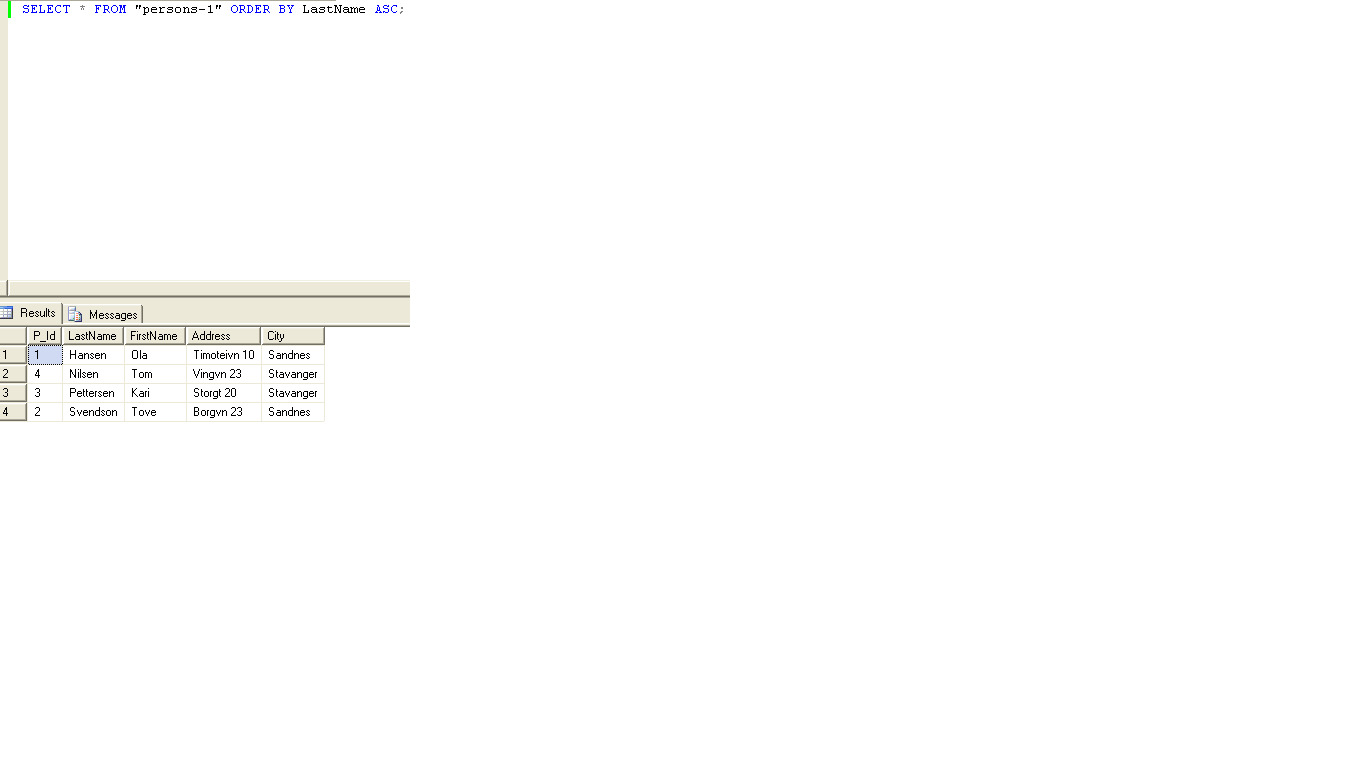
\includegraphics[scale=0.5]{figs/im-2.jpg}
			\item
				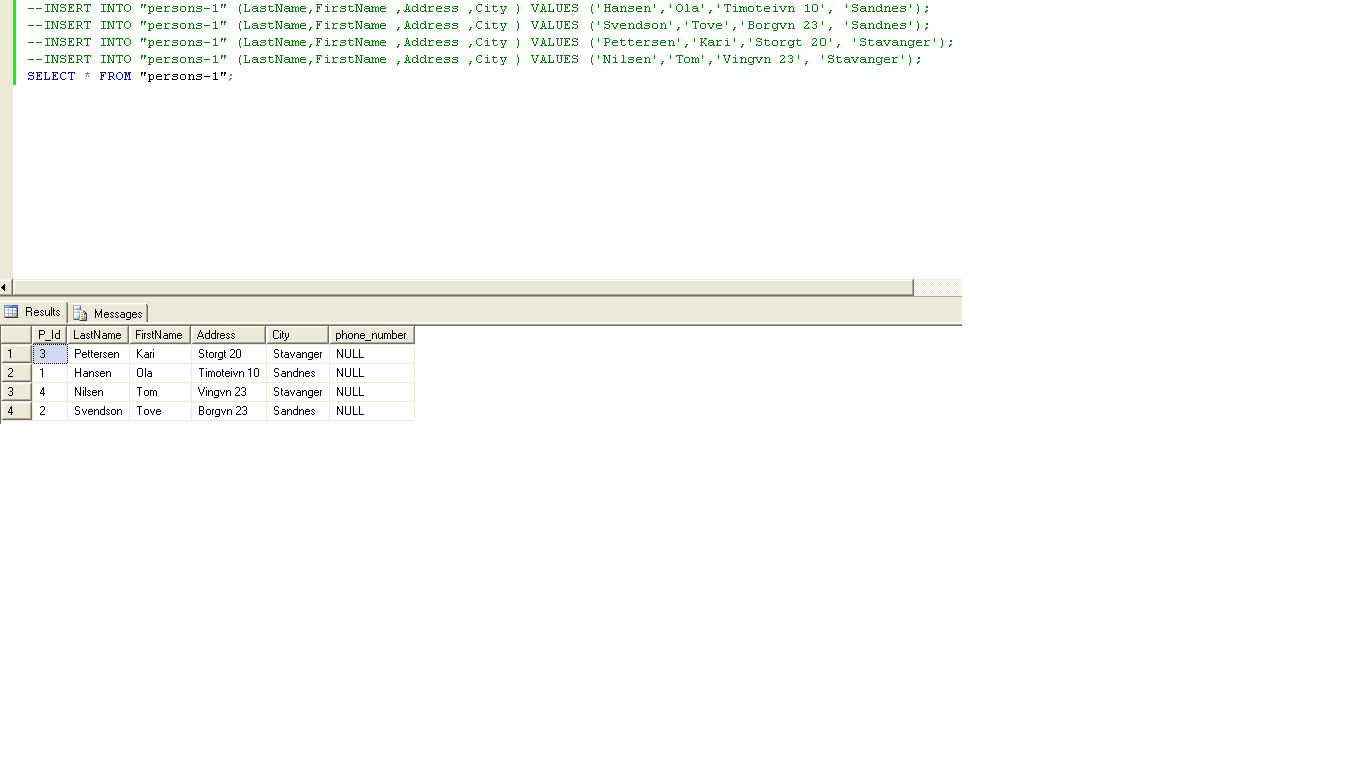
\includegraphics[scale=0.5]{figs/im-3.jpg}
			\item
				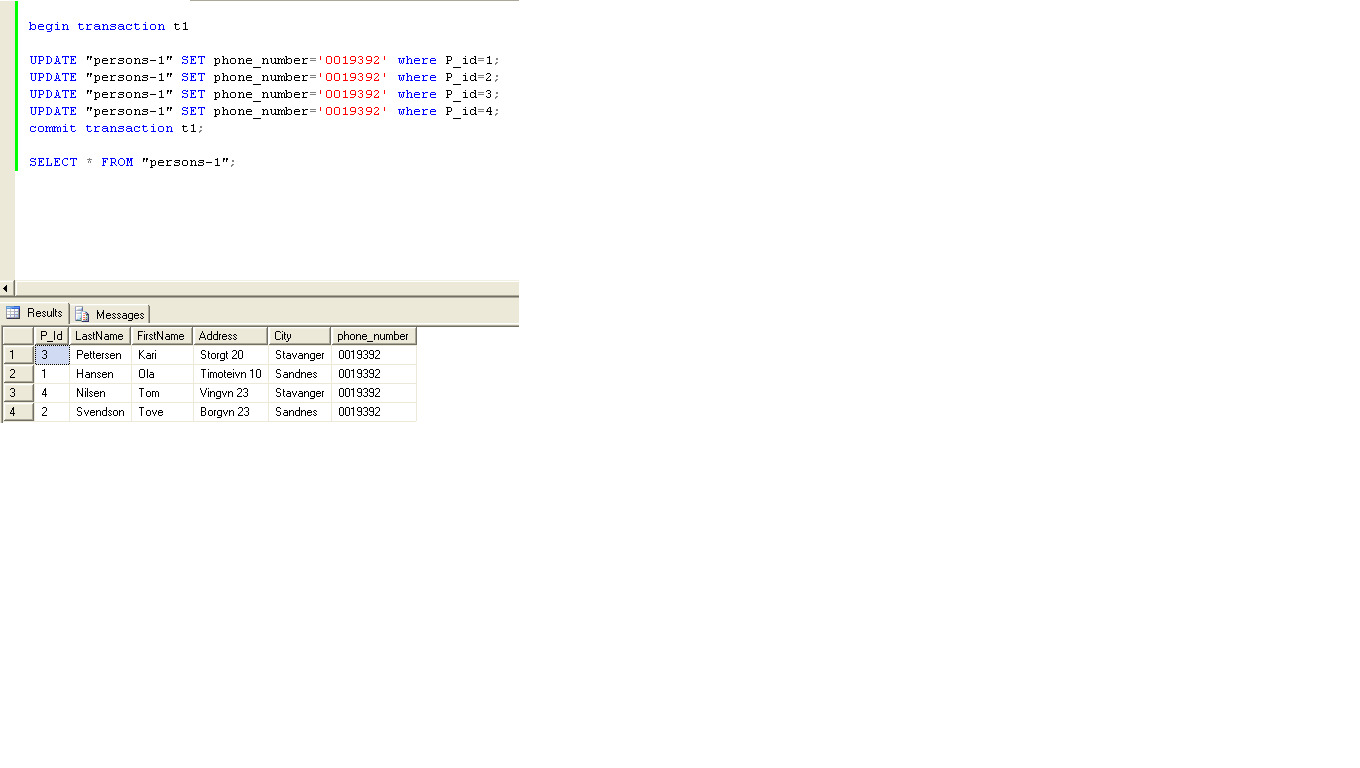
\includegraphics[scale=0.5]{figs/im-4.jpg}
			\item
				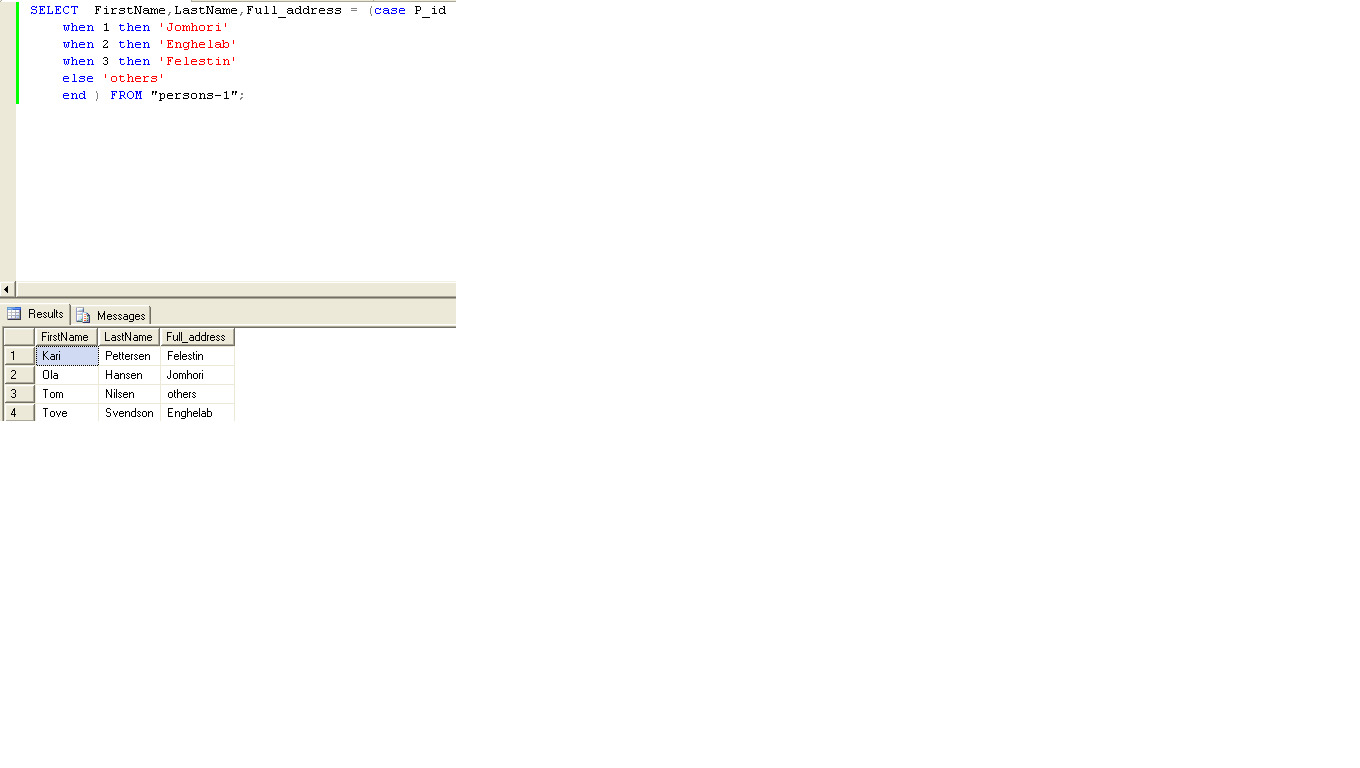
\includegraphics[scale=0.5]{figs/im-5.jpg}
			\item
				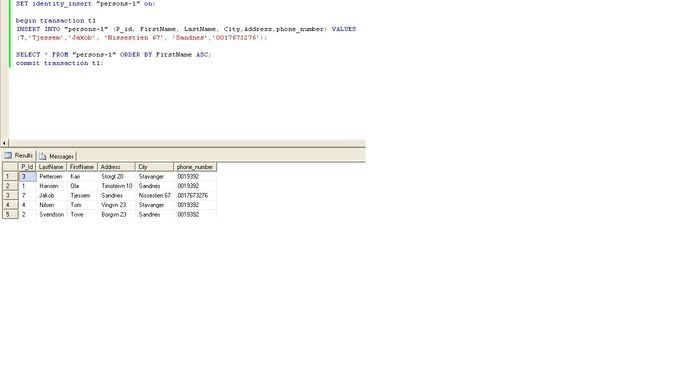
\includegraphics[scale=0.5]{figs/im-6.jpg}
			\item
				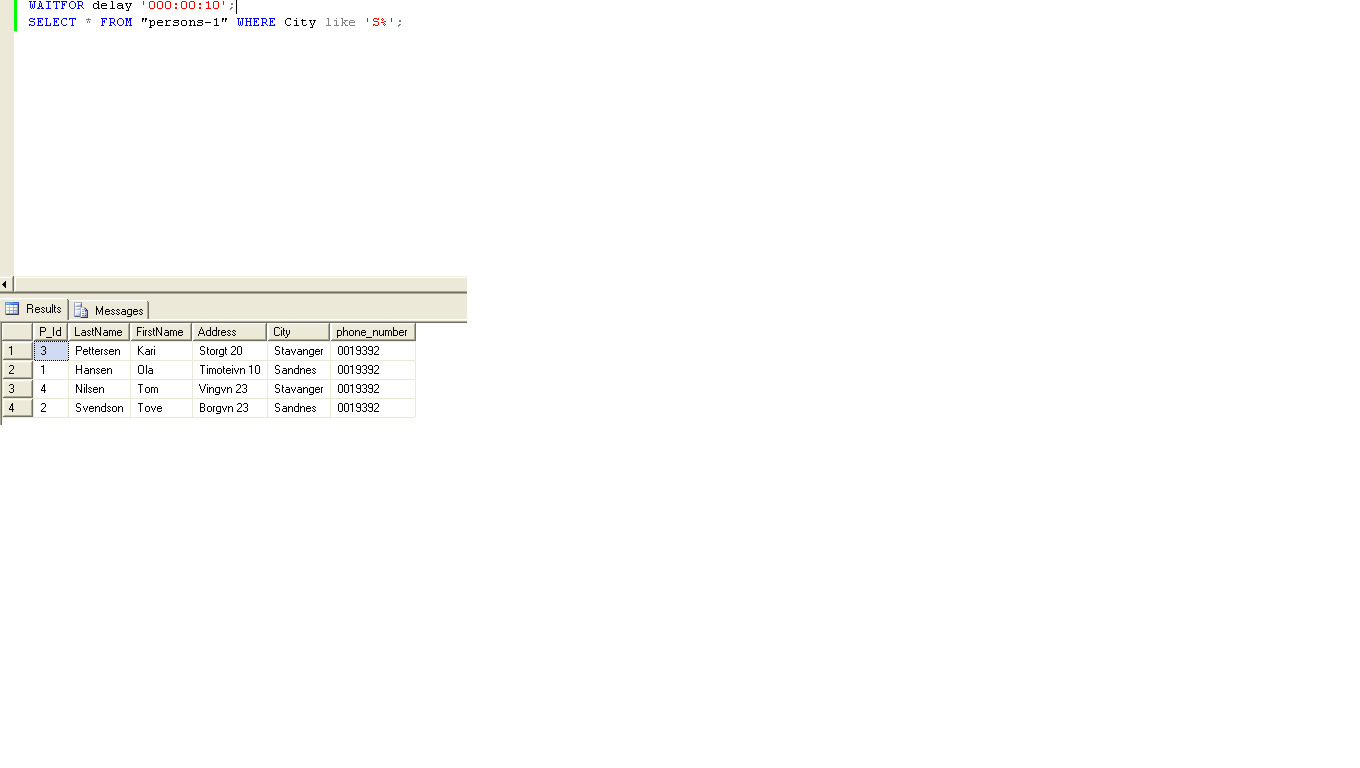
\includegraphics[scale=0.5]{figs/im-7.jpg}
			\item
				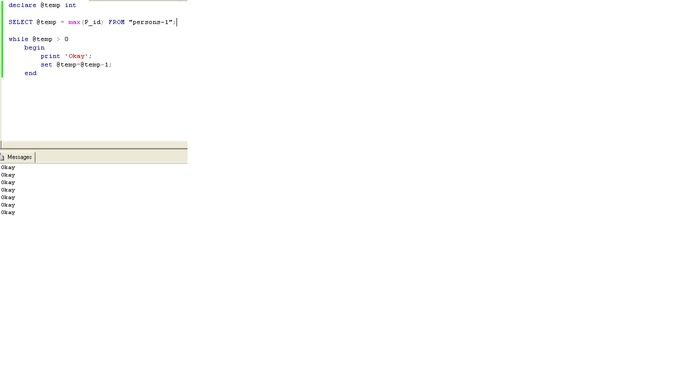
\includegraphics[scale=0.5]{figs/im-8.jpg}
			\item
				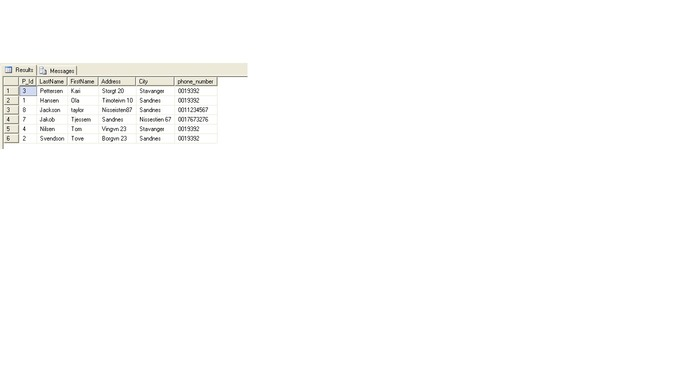
\includegraphics[scale=0.5]{figs/im-9.jpg}
		\end{enumerate}
	\item[2.]
		\begin{enumerate}
			\item
				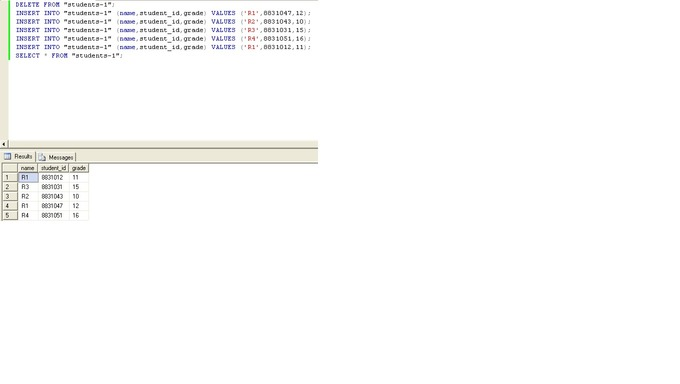
\includegraphics[scale=0.5]{figs/im-2-2.jpg}
			\item
				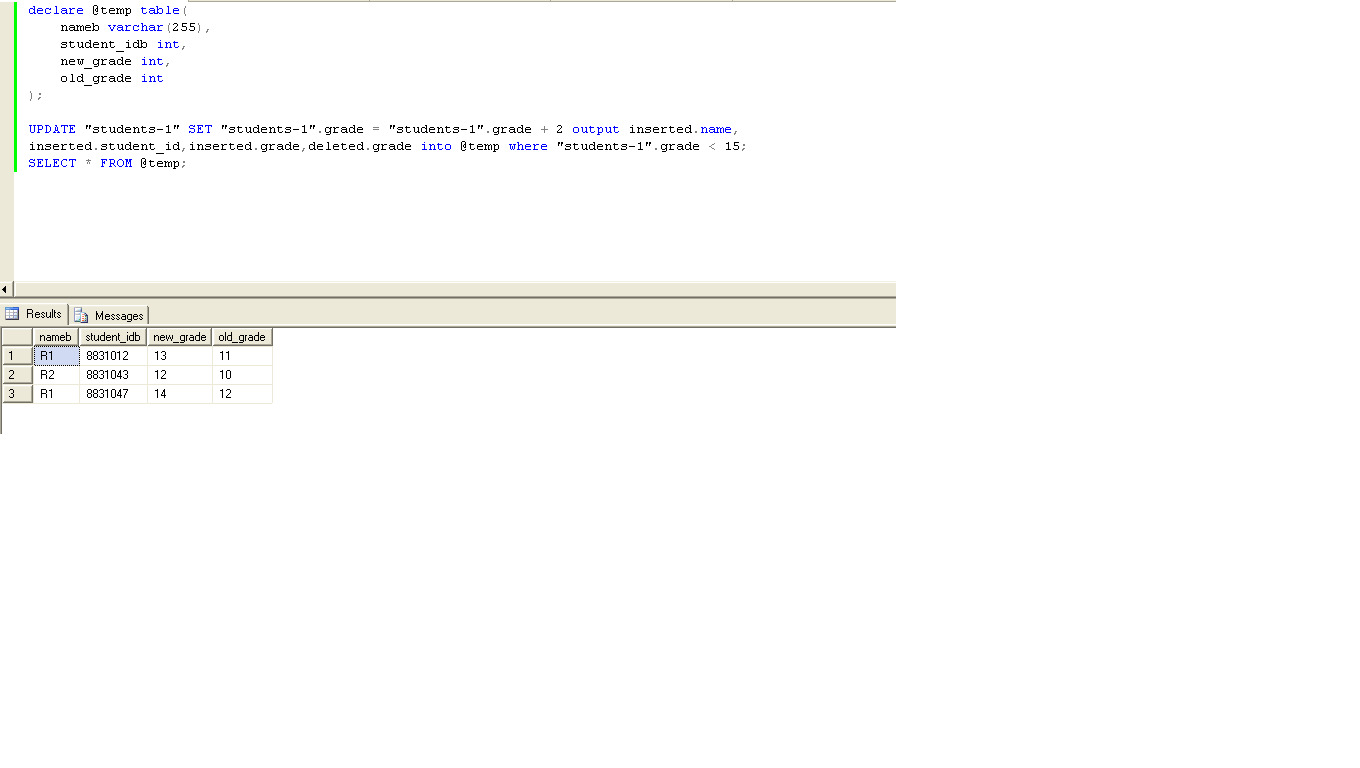
\includegraphics[scale=0.5]{figs/im-2-3.jpg}
		\end{enumerate}
\end{enumerate}
\end{document}
